\documentclass{joel_cv}
	\usepackage[colorlinks,linkcolor=red]{hyperref}
	\usepackage{enumitem}
	\usepackage{graphicx} 
	
	\begin{document}
	\pagestyle{empty}
	
	% Name, phone, email, address
	\begin{cvHeader} 
		\printName{Wentao Zhang}
		\textit{Phone:} (+1)213-255-1218 \quad \textit{E-mail:} zhan914@usc.edu
		\quad \textit{Website:} https://nsknojj.github.io
		%\printaddress{R505, CSIE Bldg., No. 1, Sec. 4, Roosevelt Rd., Taipei, Taiwan}
	\end{cvHeader}
	
	%
	% Education
	%
	
	\sectionTitle{Education}
	\begin{sectionContentSimple}{University of Southern California}{June 2017 - Present}
	\vspace{-0.2em}
		\item Master student in Computer Science % \quad -- GPA: 4.0/4.0
	\end{sectionContentSimple}
	\vspace{-0.3em}
	\begin{sectionContentSimple}{Peking University}{Sep. 2013 - July. 2017}
	\vspace{-0.2em}
		\item B.S. in Computer Science and Technology  \quad -- Major GPA: 3.65/4.0
	\end{sectionContentSimple}
	
	%
	% Experience
	%
	
	\sectionTitle{Experience}
	\parskip=0.5em
	\begin{sectionContentSimple}{Zhang Research Group, Computer Systems Lab, Cornell Univ.}{July 2016 - Sept. 2016}
		\item Research Assistant
		\vspace{-0.5em}
		\begin{itemize}
			\itemsep=-0.6em
			\item Did research on Binarized Neural Network (BNN) Inference Acceleration.
			\item Rebuilt the BNN in C++, including conv-layer, dense-layer, etc. Reduced the pipeline delay.
			\item Used Halide to optimize BNN pipeline by parallelizing loops and vectorizing computation.
			\item Compiled the BNN pipeline on x86 processor and mGPU board. Tested the performance, got a 2x speedup on average against the original BNN implementation with Lasagne.
		\end{itemize}
	\end{sectionContentSimple}
	\vspace{-0.2em}
	
	\begin{sectionContentSimple}{National Engineering Lab for Video Technology, Peking Univ.}{Apr. 2015 - June 2016}
		\item Software Development Intern
		\vspace{-0.5em}
		\begin{itemize}
			\itemsep=-0.6em
			\item Developed a video searching demo based on feature matching.
			\item Extracted the image feature at various scales and precision with OpenCV.
			\item Introduced Compact Descriptors for Visual Search (CDVS) as an efficient method extracting the video frame feature, and designed an image-to-video matching scheme.
			\item Experimented different parameter values for frame down sampling and video interval sampling to gain speedup without loss of accuracy.
			\item Wrapped the application by adding Qt GUI, including file selector, video player and frame locator.
		\end{itemize}
	\end{sectionContentSimple}
	
	%
	% Awards
	%
	
	\sectionTitle{Awards, Grants \& Honors}
	\begin{description}{}
		\parskip=0.1em
		\item{\quad} The ACM-ICPC Asia Regional Contest Mudanjiang Site 2014 Gold Medal 10th Place
		\item{\quad} International Olympiad in Informatics (IOI) 2013 China Team Selection Competition 9th Place
	\end{description}
	
	%
	%Technical Strengths
	%
	
	\sectionTitle{Technical Skills}
	\begin{description}{}
		\parskip=0em
		\item{\quad \textbf{Programming Languages:}}  C, C++, Python, Java, Assembly, SQL, MATLAB, Linux Shell, \LaTeX{}
		\item{\quad \textbf{Web Development:}} Javascript, HTML/CSS, PHP, JQuery, Tornado, Flask, Scrapy, Heritrix
		\item{\quad \textbf{Other Frameworks:}} Halide, OpenCL, OpenMP, MPICH, Hadoop, Tensorflow, OpenCV, QT
	\end{description}
	
	
	%
	% Projects
	%
	
	\sectionTitle{Projects}
	
	\parskip=0.5em
	
	\begin{sectionContentSimple}{Route Recognition Based on Coarse-grained Cellphone Location Information}{May 2017}
	\item Used multi-layer dynamic programming to retrieving the route based on simulative location data.
	\end{sectionContentSimple}
	\vspace{-0.2em}
	\begin{sectionContentSimple}{Multi-people editing plugin for Atom Text Editor}{Oct. 2015 - Dec. 2015}
	\item Involved designing communication protocols and usability testing.
	\item Independently built the server-side that retrieved JSON information from clients and transferred it.
	\item Used SQLite to implement server-side file permission management.
	\end{sectionContentSimple}
	\vspace{-0.2em}
	\begin{sectionContentSimple}{Pedestrian and Car Detection on PKUSVD Dataset}{Nov. 2015 - Dec. 2015}
	\item Applied Fast-RCNN model on PKUSVD Dataset, got 85\% precision with 80\% recall on average.
	\end{sectionContentSimple}
	\vspace{-0.2em}
	\begin{sectionContentSimple}{Image Segmentation}{June 2015}
	\item Independently implemented semi-supervised image segmentation based on min-cut algorithm.
	\end{sectionContentSimple}
	
	\sectionTitle{Publications}
	\begin{sectionContentNaive}
	
	\item Ritchie Zhao, Weinan Song, Wentao Zhang, et al. "Accelerating Binarized Convolutional Neural Networks with Software-Programmable FPGAs." In FPGA, pp. 15-24. 2017.
	
	\end{sectionContentNaive}
	% For aesthetic
	%\pagebreak
	
	
	%\sectionTitle{A Photo Taken at Brooklyn Bridge}
	%\centering 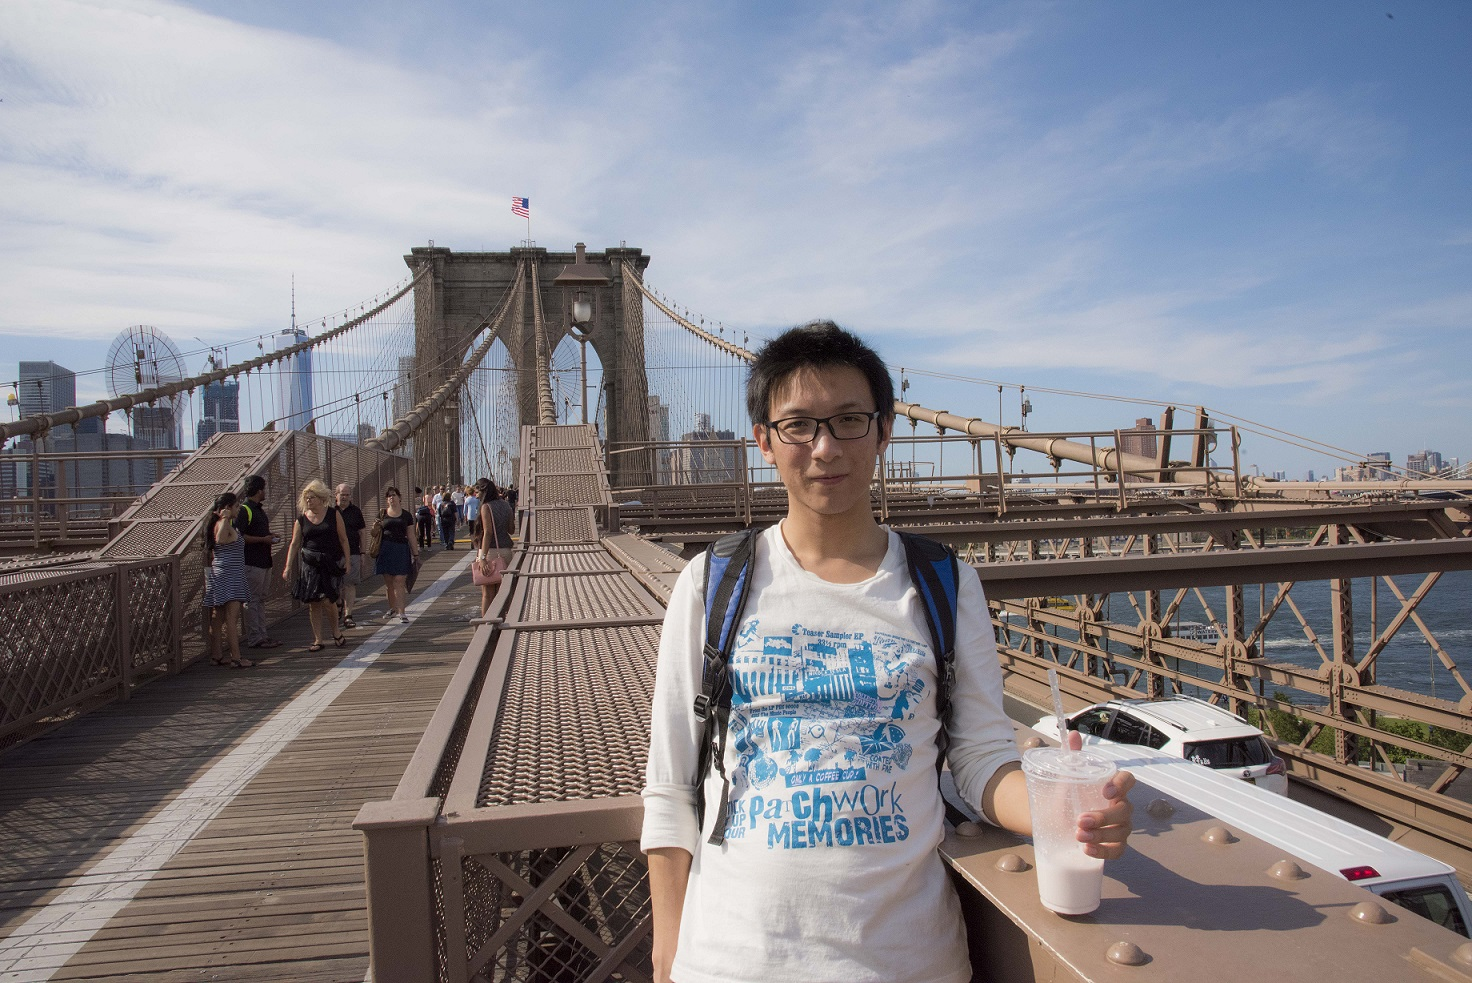
\includegraphics[height=4in]{brooklyn.jpg}
	
	\end{document}
	
	